\section{Auswertung}
\label{sec:Auswertung}
\subsection{Bestimmung der Reichweite von Alpha-Strahlung}
Es werden zwei Messungen für zwei verschiedene feste Abstände durchgeführt.
Es werden Zählrate, Druck und Channel aufgenommen.
Der Channel für die Messung bei $\SI{0}{\milli\bar}$ entspricht $\SI{4}{\mega\electronvolt}$.
Die effektive Länge wird mit Gleichung \eqref{xeff} bestimmt.
Die so erhaltenen Werte sind in Tabelle \ref{tab:mess1} aufgetragen.
\begin{table}[H]
    \caption{Messwerte für einen festen Abstand von $x_0=\SI{2}{\centi\meter}$.}
    \label{tab:mess1}
    \centering
    \begin{tabular}{S[table-format=5.0] S[table-format=1.2(0)e0] S[table-format=4.0(0)e0] S[table-format=1.2(0)e0]  }
        \toprule
        {Zählrate$/\num{120}^{-1}\si[per-mode=reciprocal]{\per\second}$} & {Energie$/\si{\mega\electronvolt}$} & {Druck$/\si{\milli\bar}$} &{effektive Länge$/\si{\centi\meter}$} \\
        \midrule
        74271 & 4.00 & 0 & 0.00\\
        73634 & 3.97 & 50 & 0.10\\
        71805 & 3.87 & 100 & 0.20\\
        69331 & 3.78 & 150 & 0.30\\
        67027 & 3.60 & 200 & 0.39\\
        64835 & 3.55 & 250 & 0.49\\
        61440 & 3.43 & 300 & 0.59\\
        33760 & 3.06 & 350 & 0.69\\
        28770 & 3.02 & 400 & 0.79\\
        41401 & 3.06 & 450 & 0.89\\
        41124 & 3.05 & 500 & 0.99\\
        33198 & 3.01 & 550 & 1.09\\
        27967 & 3.02 & 600 & 1.18\\
        20681 & 3.00 & 650 & 1.28\\
        15966 & 2.99 & 700 & 1.38\\
        9472 & 2.99 & 750 & 1.48\\
        6076 & 2.99 & 800 & 1.58\\
        2561 & 3.01 & 850 & 1.68\\
        937 & 2.99 & 900 & 1.78\\
        397 & 2.98 & 950 & 1.88\\
        99 & 3.00 & 1000 & 1.97\\
        \bottomrule
    \end{tabular}
\end{table}
\noindent Die Zählrate wird in Abbildung \ref{fig:c1} gegen die effektive Länge aufgetragen.
Es wird eine Reggressionsgerade mit SciPy/Python nach der Funktionsvorschrift
\begin{equation*}
  f(x) = mx +b
\end{equation*}
erstellt.
\begin{figure}[H]
  \centering
  \includegraphics{build/counts1.pdf}
  \caption{Lineare Reggression für die Zählrate in Abhängigkeit der effektiven Länge.}
  \label{fig:c1}
\end{figure}
\noindent Dabei ergeben sich folgenede Parameter:
\begin{equation*}
  m =\SI{-384\pm29}{\per\second\per\centi\meter}
\end{equation*}
und
\begin{equation*}
  b =\SI{667\pm27}{\per\second}.
\end{equation*}
Die mittlere Reichweite ergibt sich dann als Schnittpunkt der Regressionsgeraden mit der Horizontalen bei $y=\SI{309.46}{\per\second}$.
Die mittlere Reichweite kann, dann durch umstellen der Funktionsvorschrift, mit
\begin{equation*}
  R_m=\frac{\SI[per-mode=reciprocal]{309.46}{\per\second}-b}{m}
\end{equation*}
bestimmt werden.
Der Fehler der mittleren Reichweite wird mit Gaußscher Fehlerfortpflanzung nach
\begin{equation*}
  \sigma_R = \sqrt{\left(\frac{b-\SI{309.46}{\per\second}}{m^2}\sigma_m\right)^2 +\left(\frac{1}{m}\sigma_b\right)^2}
\end{equation*}
berrechnet.
Der so erhaltene Wert beträgt $R_m= \SI{0.93\pm0.1}{\centi\meter}$.
Damit lässt sich nach Gleichung \eqref{Rm} eine Energie von $E_{\alpha} = \SI{0.45}{\mega\electronvolt}$ bestimmen.
Die Energie wird in Abbildung \ref{fig:e1} als Funktion der effektiven Länge aufgetragen.
Es wird eine Reggressionsgerade nach der Vorschrift
\begin{equation*}
  f(x) = mx + b
\end{equation*}
durch die Messwerte gezogen.
Für die Regressionsrechnung wird nur der lineare Anteil der Messwerte verwendet.
\begin{figure}[H]
  \centering
  \includegraphics{build/energie1.pdf}
  \caption{Lineare Reggression für die Energie in Abhängigkeit der effektiven Länge.}
  \label{fig:e1}
\end{figure}
\noindent Der Energieverlust $-\frac{dE}{dx}$ kann dann als Steigung der Regression bestimmt werden.
Damit ergibt sich ein Energieverlust von
\begin{equation*}
  -\frac{dE}{dx} = \SI{-0.52\pm0.07}{\mega\electronvolt\per\centi\meter} .
\end{equation*}
Analog wird für den zweiten Abstand vorgegangen.
Die Messwerte sowie Energien und effektive Längen sind in Tabelle \ref{tab:mess2} aufgetragen.
\begin{table}[H]
    \caption{Messwerte für einen festen Abstand von $x_0=\SI{1.5}{\centi\meter}$.}
    \label{tab:mess2}
    \centering
    \begin{tabular}{S[table-format=6.0] S[table-format=1.2(0)e0] S[table-format=4.0(0)e0] S[table-format=1.2(0)e0]  }
        \toprule
        {Zählrate$/\num{120}^{-1}\si{\per\second}$} & {Energie$/\si{\mega\electronvolt}$} & {Druck$/\si{\milli\bar}$} &{effektive Länge$/\si{\centi\meter}$} \\
        \midrule
        148139 & 4.00 & 0 & 0.00\\
        150632 & 3.93 & 50 & 0.07\\
        149256 & 3.85 & 100 & 0.15\\
        143513 & 3.56 & 150 & 0.22\\
        139419 & 3.46 & 200 & 0.30\\
        145173 & 3.56 & 250 & 0.37\\
        136922 & 3.29 & 300 & 0.44\\
        134960 & 3.20 & 350 & 0.52\\
        133809 & 3.15 & 400 & 0.59\\
        138624 & 3.22 & 450 & 0.66\\
        138244 & 3.19 & 500 & 0.74\\
        130125 & 2.95 & 550 & 0.81\\
        131421 & 2.95 & 600 & 0.89\\
        125958 & 2.79 & 650 & 0.96\\
        123717 & 2.72 & 700 & 1.04\\
        121739 & 2.67 & 750 & 1.11\\
        120083 & 2.59 & 800 & 1.18\\
        117426 & 2.49 & 850 & 1.26\\
        114320 & 2.45 & 900 & 1.33\\
        112018 & 2.42 & 950 & 1.41\\
        104394 & 2.36 & 1000 & 1.48\\
        \bottomrule
    \end{tabular}
\end{table}
\noindent In Abbildung \ref{fig:c2} ist die Zählrate gegen die effektive Länge aufgetragen, zusätzlich ist noch eine lineare Ausgleichsgerade eingezeichnet.
\begin{figure}[H]
  \centering
  \includegraphics{build/counts2.pdf}
  \caption{Lineare Reggression für die Zählrate in Abhängigkeit der effektiven Länge.}
  \label{fig:c2}
\end{figure}
\noindent Für die Ausgleichsrechnung ergeben sich die Parameter
\begin{equation*}
  m = \SI{-204\pm17}{\per\second\per\centi\meter}
\end{equation*}
und
\begin{equation*}
  b = \SI{1254\pm12}{\per\second}   .
\end{equation*}
Die mittlere Reichweite berechnet sich durch den Schnittpunkt der Ausgleichsgerade mit der Horizontalen am Punkt $y=\SI{617.25}{\per\second}$.
Es ergibt sich für die mittlere Reichweite:
\begin{equation}
  R_m= \SI{3.12\pm0.27}{\centi\meter} 
\end{equation}
Ihr Fehler berrechnet sich über die Gaußsche Fehlerfortpflanzung, gemäß:
\begin{equation*}
    \sigma_R = \sqrt{\left(\frac{b-\SI{617.25}{\per\second}}{m^2}\sigma_m\right)^2 +\left(\frac{1}{m}\sigma_b\right)^2} 
\end{equation*}
Der zugehörige Energiewert beträgt $E_{\alpha}=$FEHLT.
Die Energie wird in Abbildung \ref{fig:e2} als Funktion der effektiven Länge aufgetragen.
Es wird eine Reggressionsgerade nach der Vorschrift
\begin{equation*}
  f(x) = mx + b
\end{equation*}
durch die Messwerte gezogen.
Damit ergibt sich für den Energieverlust ein Wert von
\begin{equation*}
  -\frac{dE}{dx} =\SI{-1.10\pm0.04}{\mega\electronvolt\per\centi\meter} .
\end{equation*}

\begin{figure}[H]
  \centering
  \includegraphics{build/energie2.pdf}
  \caption{Lineare Reggression für die Energie in Abhängigkeit der effektiven Länge.}
  \label{fig:e2}
\end{figure}

\subsection{Statistik des radioaktiven Zerfalls}
Die Messwerte sind in Tabelle \ref{tab:pos} eingetragen.
\begin{table}[H]
    \caption{Messwerte für die Statistik des radioaktiven Zerfalls.}
    \label{tab:pos}
    \centering
    \begin{tabular}{S[table-format=4.0] S[table-format=4.0] S[table-format=4.0] S[table-format=4.0] S[table-format=4.0]  }
        \toprule
        {Zählrate$/\num{10}^-1\si{\per\second}$} & {Zählrate$/\num{10}^-1\si{\per\second}$}  & {Zählrate$/\num{10}^-1\si{\per\second}$} & {Zählrate$/\num{10}^-1\si{\per\second}$}  & {Zählrate$/\num{10}^-1\si{\per\second}$}  \\
        \midrule
        3378 & 3677 & 3355 & 3590 & 3310\\
        3674 & 3550 & 3367 & 3500 & 3693\\
        3605 & 3602 & 3419 & 3372 & 3581\\
        3447 & 3411 & 3549 & 3458 & 3670\\
        3533 & 3583 & 3673 & 3479 & 3474\\
        3445 & 3446 & 3586 & 3512 & 3717\\
        3515 & 3570 & 3632 & 3672 & 3606\\
        3639 & 3667 & 3762 & 3557 & 3479\\
        3602 & 3546 & 3467 & 3614 & 3559\\
        3410 & 3786 & 3468 & 3624 & 3819\\
        3754 & 3384 & 3460 & 3404 & 3457\\
        3760 & 3744 & 3373 & 3429 & 3699\\
        3620 & 3475 & 3537 & 3605 & 3542\\
        3603 & 3624 & 3791 & 3711 & 3446\\
        3476 & 3488 & 3540 & 3791 & 3526\\
        3407 & 3473 & 3667 & 3620 & 3498\\
        3674 & 3783 & 3806 & 3551 & 3565\\
        3871 & 3602 & 3858 & 3487 & 3648\\
        3576 & 3395 & 3680 & 3590 & 3704\\
        3696 & 3513 & 3508 & 3512 & 3617\\
        \bottomrule
    \end{tabular}
\end{table}
\noindent Die Zählraten sind in zwei Histogrammen aufgetragen.
In Abbildung \ref{fig:pos} ist zusätzlich eine Poissonverteilung aufgetragen und in Abbildung \ref{fig:gauß} eine Gaußverteilung.
Der Mittelwert der Zählrate beträgt $\bar{N}= \num{357.19}$ und die Varianz $\sigma_N = \num{156.326}$.
Für die Poissonverteilung wird die Gleichung
\begin{equation}
  P(N)=\frac{\lambda^N \exp(-\lambda)}{N!}
\end{equation}
verwendet.
Die Gaußverteilung wird mit der Gleichung
\begin{equation}
  G(N) = \frac{A}{\sigma_N \sqrt{2\pi}} \exp\left(-\frac{1}{2}\left(\frac{N-\bar{N}}{\sigma_N}\right)\right)
\end{equation}
erzeugt.
\begin{figure}[H]
  \centering
  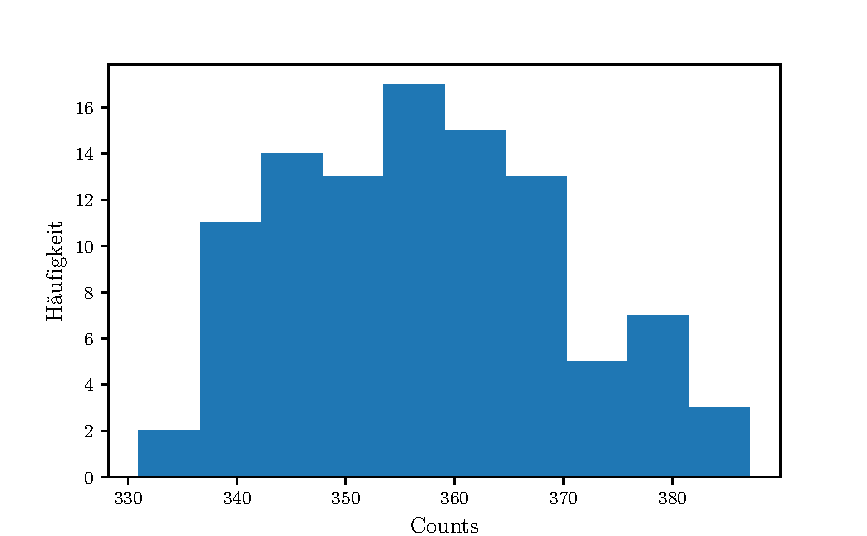
\includegraphics{build/PlotPoisson.pdf}
  \caption{Histogramm für die Statistik des radioaktiven Zerfalls mit Poissonverteilung.}
  \label{fig:pos}
\end{figure}
\begin{figure}[H]
  \centering
  \includegraphics{build/PlotGauss.pdf}
  \caption{Histogramm für die Statistik des radioaktiven Zerfalls mit Gaußverteilung.}
  \label{fig:gauß}
\end{figure}
